\subsection{Процессы инициации, планирования, реализации проекта}

\textit{Инициация проекта}, являясь одной из важнейших его фаз, закладывает фундамент успеха всего проекта.
Здесь определяются основные цели проекта, анализируются стратегические риски, выделяются ключевые участники проекта, определяются общие принципы организации управления проектом.

В состав процессов инициации входят:
\begin{itemize}
	\item  разработка устава проекта;
	\item  анализ заинтересованных сторон;
	\item  сбор требований;
	\item  стартовое совещание по проекту.
\end{itemize}

Основными задачами в ходе инициации проекта являются:
\begin{itemize}
	\item понимание основных заинтересованных сторон проекта, их интере­сов и ожиданий от проекта и его результатов;
	\item сбор требований от заказчика и иных заинтересованных сторон;
	\item формальный авторизованный старт проекта путем выпуска до­кумента <<Устав проекта>> и проведения стартового совещания по
	проекту.
\end{itemize}

Рассмотрим процессы инициации проекта более подробно.

Разработка устава проекта.
Целью разработки устава проекта является авторизация и формализа­ция проекта путем четкого очерчивания границ проекта, документиро­вания его целей и результатов, определения менеджера проекта, зоны его ответственности и полномочий.
Устав проекта должен связать проект со стратегическими целями организации, обосновать его необходимость, определить его содержа­ние и ответственных за реализацию.

Целью устава проекта, как исходного интеграционного документа является обеспечение однозначного понимания и фиксация:
\begin{itemize}
	\item  обоснование инициации проекта;
	\item  цели и результаты проекта;
	\item  описание и структуру продукта проекта;
	\item ожидания ключевых участников проекта;
	\item критерии успеха проекта;
	\item фамилию менеджера проекта и зону его ответственности в проекте;
	\item основные принципы организации проекта и управления им.
\end{itemize}

Устав проекта --- документ, разработка которого направлена на обеспечение следующих результатов:
\begin{itemize}
	\item авторизацию проекта;
\item определение проекта;
\item назначение менеджера проекта и распределения ролей основных участников проекта.
\end{itemize}

Результатами процесса разработки устава проекта являются однознач­ное понимание содержания проекта всеми его участниками и автори­зация начала проекта лицами, принимающими решение \cite[135--137]{polkovnikov}

Анализ заинтересованных сторон.
Целью анализа заинтересованных сторон является понимание возмож­ных зон воздействия на проект со стороны его участников и внешних заинтересованных сторон путем выявления основных лиц, групп и организаций, имеющих прямые или косвенные интересы в проекте.

Заинтересованные стороны (стейкхолдеры) в проекте существуют независимо от нашего желания.
Если бы их не было, проект никогда бы не состоялся.
При этом и х интересы весьма различаются.
Одни заинтересованные стороны проект запускают, продвигают к успеху, другие стороны имеют иные интересы.

Интересы по отношению к проекту могут быть:
\begin{itemize}
	\item положительными или отрицательными;
	\item прямыми или косвенными;
	\item явными и неявными (скрытыми).
\end{itemize}

Действия заинтересованных сторон иногда способствуют успеху проекта, а иногда --- нет.
Заинтересованные стороны будут влиять на окружение проекта (см. рисунок \ref{fig:okuzhenie}), создавая для менеджера проекта либо позитивные условия, либо серьезные препятствия для успеха проекта.

\begin{figure}[h]
	\centering
	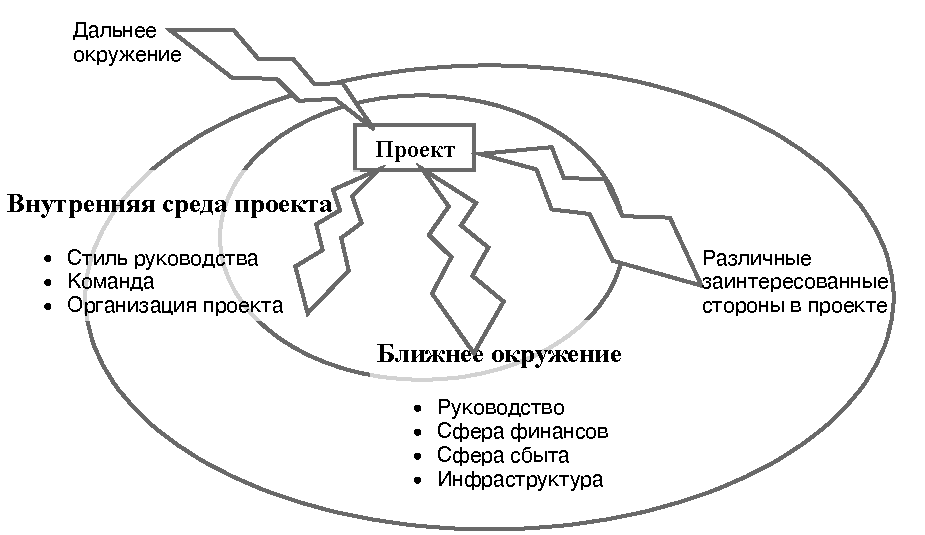
\includegraphics[width=\linewidth]{okruzh}
	\caption{Окружение проекта}
	\label{fig:okuzhenie}
\end{figure}

Выделяют ближнее и дальнее окружение проекта.
В ближнем окружении основными заинтересованными сторонами являются руко­водство организации, представители функциональных подразделений,
сотрудники, в дальнем --- конкуренты, органы власти, представители общественных организаций.

В ходе анализа заинтересованных сторон в проекте рекомендуется выделить основные группы заинтересованных сторон и понять их ин­тересы.
Это требуется:
\begin{itemize}
	\item для назначения явных заинтересованных сторон (участников про­екта) на роли, соответствующие их интересам;
	\item согласования с ключевыми внутренним и (а иногда и внешними) заинтересованными сторонами целей и результатов проекта;
	\item выявления угроз и зон риска со стороны заинтересованных сторон, негативно настроенных по отношению к проекту;
	\item определения потенциальных возможностей (в том числе дополни­тельных), возникающих в случае активного привлечения соответ­ствующих заинтересованных сторон;
	\item установления информационных потребностей заинтересованных сторон и дальнейшего включения их в коммуникационное поле проекта.
\end{itemize}

Результатами процесса анализа заинтересованных сторон являются готовность менеджера и команды проекта к влиянию, оказываемому на проект различными заинтересованными сторонами, и минимизация негативных эффектов этого влияния.

Заинтересованные стороны и их интересы могут быть отражены в Реестре заинтересованных сторон.
Для каждой заинтересованной стороны в этом документе полезно зафиксировать:
\begin{itemize}
	\item имя человека или название группы, представляющих заинтересо­ванную сторону;
	\item отношение заинтересованной стороны к проекту (положительное, отрицательное, нейтральное);
	\item силу возможного влияния на проект;
	\item степень информированности о проекте, его целях и текущем со­стоянии;
	\item дополнительные условия, при которых отношение к проекту может измениться.
\end{itemize}

По итогам анализа заинтересованных сторон проекта могут быть внесены изменения в существующие проектные документы: Устав,
План проекта и др. \cite[141--143]{polkovnikov}.

Сбор требований.
Целью процесса сбора требований является достижение более пол­ного, четкого и однозначного понимания целей и результатов проекта, а также ожиданий заказчика и иных заинтересованных сторон в ча­сти, касающейся функциональных, технических, пользовательских и иных характеристик продукта проекта.

Необходимо получить, понять, проанализировать и документаль­но зафиксировать требования основных заинтересованных сторон, которые могут повлиять на содержание проекта и организацию его выполнения.

Требования могут относиться к любым аспектам проекта:
\begin{itemize}
	\item целям и результатам;
	\item продукту проекта и его характеристикам;
	\item жизненному циклу проекта, этапам или составным элементам проекта;
	\item условиям реализации проекта и правилам выполнения отдельных работ;
	\item схемам финансирования или привлечения средств;
	\item условиям взаимодействия между участниками;
	\item правилам приемки продукта или сдачи результатов промежуточ­ных этапов и др.
\end{itemize}

Чаще всего требования распространяются на цели и результаты, а также на продукт проекта.
Основную роль в определении требова­ний играют ключевые заинтересованные стороны, в первую очередь заказчик.

Кроме того, при определении требований к продукту проекта важ­ным является понимание таких заинтересованных сторон, как поль­зователи, будущие покупатели (клиенты), эксплуатирующая орга­низация.

Результатом процесса сбора требований должна стать минимизация дополнительных требований и пожеланий заказчика по отношению к продукту проекта и проекту в целом, возникающих в ходе его реализа­ции.
В идеальной ситуации их не должно быть совсем. Как следствие, это должно привести к минимизации внесения изменений в проект на более поздних этапах.

Иногда по итогам процесса сбора требований создается документ Требования к продукту или Технические требования к проекту.
В зависимости от содержания проекта название документа может из­меняться \cite[143--144]{polkovnikov}.

Стартовое совещание по проекту.
Целью стартового совещания по проекту является информирование всех заинтересованных сторон проекта об основных решениях, приня­тых в ходе инициации проекта, и согласование с ними утверждаемых проектных документов.

Эффективно проведенное стартовое совещание может дать мощный импульс всему проекту и задать верное направление работе команды проекта.

В повестку дня стартового совещания по проекту рекомендуется включить следующие пункты:
\begin{itemize}
	\item представление менеджера проекта, куратора и заказчика;
	\item знакомство участников;
	\item идея и замысел проекта, предпосылки и обоснование его запуска;
	\item основные положения Устава проекта;
	\item распределение ролей в команде проекта и степени загрузки участ­ников в проекте;
	\item принципы организации и взаимодействия в проекте.
\end{itemize}

Присутствие на стартовом совещании по проекту куратора, заказ­чика и иных важных участников поднимет статус проекта и статус менеджера проекта в глазах членов проектной команды.

Согласование с командой целей и результатов, принципов работы и взаимодействия позволит вовлечь участников в процесс управления и принятия решений по проекту, что должно повысить их ответствен­ность и мотивацию.

Результатом стартового совещания по проекту должно стать четкое, общее и одинаковое понимание участниками проекта его целей и за­дач, текущего статуса, системы организации проекта и своего места в команде начинающегося проекта \cite[145]{polkovnikov}.

Начало проекта закладывает фундамент всех его успехов.
Ошибки, допущенные в ходе инициации, обязательно напомнят о себе в даль­нейшем.
К числу самых распространенных ошибок, случающихся в начальной стадии проекта, относятся:
\begin{itemize}
	\item нечеткое понимание целей и границ проекта;
	\item неформализованный подход к запуску проекта;
	\item необоснованный запуск проекта.
\end{itemize}

\textit{Планирование проекта} --- процесс поиска и расчета оптимального способа достижения целей проекта.

В ходе планирования необходимо по воз­можности четко ответить на вопросы: кто, когда, как и какие работы должен выпол­нить для достижения целей проекта.

Ответы на эти вопросы ищутся и находятся в ходе последовательной разработки Плана проекта --- единого сводного документа, со­держащего результаты планирования основ­ных функциональных областей проекта:
\begin{itemize}
	\item сроков;
	\item стоимости;
	\item персонала;
	\item поставок;
	\item рисков;
	\item коммуникаций и др.
\end{itemize}

Процессы планирования --- процессы, осуществляемые для тщательного определения содержания проекта, разработки плана управления проектом и идентификации и составления расписания операций проекта, которые будут проводиться в рамках проекта.

Планированию в проекте подлежит большое число аспектов:
\begin{itemize}
	\item сроки;
	\item деньги;
	\item персонал;
	\item поставки;
	\item качество;
	\item коммуникации.
\end{itemize}

Центральным в планировании является процесс календарного плани­рования и разработки реалистичного расписания проекта.
Результаты календарного планирования используются в дальнейшем при плани­ровании других элементов проекта.

Бюджет проекта --- директивный документ, представляющий собой график планируемых расходов и доходов, распределенных по статьям в рамках проекта.
Погрешность, допустимая в бюджете, зависит от вида бюджета и от его назначения.

План персонала содержит информацию о том, кто, когда и какие за­дачи будет выполнять в проекте, а также какая роль делегирована тому или иному члену команды управления проектом.
Организацион­ная структура четко определит роли участников проекта и условия их подчиненности.

План поставок может быть отдельным документом, а может быть частью календарного плана.
При любых условиях он четко связан с календарным планом проекта, содержит информацию о сроках и ис­полнителях работ, отданных на подряд внешним организациям.

Реестр рисков --- документ, содержащий информацию о рисках проекта.
Помимо данных о причинах и сущности рисков в нем долж­ны содержаться конкретные планы действий по каждому выявленно­му риску.

Все планы по отдельным функциональным областям сводятся в единый план проекта.

Процессы планирования должны закончиться фиксацией базово­го плана --- эталонного плана, который будет основой для контро­ля выполнения проекта.
С данными базовых планов будут сверяться результаты фактического выполнения работ проекта и вычисляться отклонения от плана \cite[174--175]{polkovnikov}.

Планы проекта, зафиксированные в процессе планирования , должны быть выполнены.
Для их выполнения привлекаются люди , подразде­ления и целые организации.
Менеджер проекта организует распре­деление заданий между исполнителями , привлекает необходимые ре­сурсы , обеспечивает своевременное финансирование отдельных этапов и работ проекта.

Можно выделить несколько основных групп задач в составе про­цессов реализации:
\begin{itemize}
	\item работу с людьми (с командой, с заказчиком, с заинтересованными сторонами);
	\item работу с внешними организациями (с подрядчиками, с разреши­тельными, лицензирующими и другими органами ) ;
	\item работу с информацией (сбор , анализ , распространение и проч.).
\end{itemize}

При этом все процессы взаимосвязаны.
Выходы одного процесса являются входами другого .

Любой проект требует координации.
Большое число исполнителей , технологическая сложность , уникальность целей и условий их дости­жения могут значительно усложнить выполнение проекта.


Процессы исполнения проекта --- процессы, применяемые для выполнения работ, указанных в плане управления проектом, для достижения целей проекта, указанных в описании содержания проекта.

Набор команды проекта.
Целью процесса набора команды проекта является привлечение к проекту специалистов необходимой квалификации и формирование из них рабочей группы ( групп) для исполнения работ проекта.

Обычно набор команды проекта осуществляется путем привле­чения внешних и внутренних специалистов .
Внешние специалисты привлекаются в проект на условиях подряда или трудового догово­ра, сотрудники родительской организации --- на условиях полной или частичной занятости .

В случае привлечения специалистов на условиях частичной заня­тости формируется матричная организационная структура, предпола­гающая двойное подчинение сотрудника.
Он подчиняется как своему линейному руководителю , так и менеджеру проекта.
В таком случае необходимо определить и зафиксировать степень привлечения (за­грузку) исполнителя в проекте.
Она может быть определена в про­центах рабочего времени , либо в рабочих часах, либо иным способом, например сдельно.

В группе исполнителей , привлеченных к проекту , должны быть распределены роли , четко определены зоны ответственности и пол­номочий.
Каждый должен понимать свое место и задачи в группе и проекте в целом .
Задачи проекта должны быть согласованы и распре­делены между исполнителями согласно расписанию проекта.

Результатом процесса набора команды должно стать создание группы сотрудников , привлеченных к выполнению работ проекта.

Результирующим документом процесса может стать список специа­листов , которые будут привлечены в команду проекта, с указанием их роли и степени загрузки в проекте.

Выбор поставщиков.
Большое число работ в проекте выполняется силами внешних испол­нителей .
Различные исполнители и поставщики могут выполнить ра­боты с различными качеством, стоимостью и в различные сроки .

Целью процесса выбора поставщиков является привлечение к про­екту наиболее подходящих внешних исполнителей исходя из требований проекта к качеству , срокам и стоимости этих работ путем конку­рентного выявления их из множества претендентов.

Выбор поставщиков часто проводится в виде конкурса (тендера) .
В случае привлечения поставщиков к выполнению государственного заказа правила проведения тендера регулируются законодательно.
Федеральный закон четко определяет сроки , условия и технологию выбора поставщиков.
Частные компании могут организовывать кон­курс между поставщиками по своим правилам .

Компания --- организатор конкурса должна подготовить комплект документации , содержащий исходную информацию о технологических, коммерческих , организационных и иных характеристиках объекта и предмета конкурса (торгов) , а также о его условиях и процедуре .

При выборе поставщиков могут применяться различные способы оценки их предложений (оферт) :
\begin{itemize}
	\item системы балльных оценок ;
	\item системы ранжирования;
	\item системы экспертной оценки и др .
\end{itemize}

Иногда компания-заказчик заранее определяет список поставщиков, с которыми она потенциально готова работать, и тендерное состязание организуется только между ними.
Списки аттестованных поставщи­ков формируют подразделения , ответственные за закупки и поставки , путем предварительной оценки и ранжирования претендентов .

Результатом процесса должен стать перечень поставщиков и подряд­чиков , которые будут выполнять определенные работы в проекте .

Выходными документами процесса являются договоры на выпол­нение работ проекта, заключенные с соответствующими организа­циями.

Обеспечение качества.
Целью процесса обеспечения качества является выполнение и дости­жение всех показателей качества, предъявляемых к продукту и ре­зультатам проекта.

Обеспечение качества --- это управленческий процесс , направлен­ный на практическую реализацию одного из главных постулатов тео­рии управления качеством : <<эффективнее контролировать процесс, чем итоговый результат>>.

Основная задача менеджера проекта заключается в четкой фор­мализации основных управленческих и производственных процессов проекта и в аккуратнейшем их выполнении .
Проработка и документи­рование процессов без дальнейшего их применения бесполезны.
Необходимо обучить персонал и установить систему аудита выполнения процедур в проекте.

Результатом выполнения процесса обеспечения качества должна стать система подходов , методов и процедур, гарантирующая выполнение и достижение всех показателей качества, зафиксированных в ходе про­цесса планирования качества.

Координация работ и исполнителей.
Целью процесса координации работ и исполнителей является обес­печение четкого и эффективного взаимодействия участников в ходе выполнения работ проекта.

Координация работ и исполнителей включает:
\begin{itemize}
	\item распределение заданий между исполнителями согласно плану про­екта;
	\item определение приоритетов задач ;
	\item согласование рабочих вопросов с функциональными руководите­лями, представителями внешних организаций;
	\item разрешение спорных и конфликтных ситуаций ;
	\item информирование команды проекта о достигнутых результатах , об изменениях в проекте ;
	\item информационную, консультационную , управленческую и иную поддержку членов команды проекта и др .
\end{itemize}

Входными данными для процесса координации являются практи­чески все результаты процессов планирования, а также обратная связь с большим числом процессов организации исполнения .
Планирование является центральным в группе процессов организации исполнения проекта.

Результатом процесса координации работ и исполнителей должно стать эффективное , бесконфликтное выполнение работ проекта со­гласно утвержденному плану проекта.

Управление ожиданиями заинтересованных сторон.
Целью процесса управления ожиданиями заинтересованных сторон является обеспечение адекватных предположений заинтересованных сторон по поводу продукта проекта, его характеристик, сроков и стои­мости, а также об иных параметрах проекта, предотвращение фор­мирования у них завышенных или нереалистичных представлений о проекте .

Соответствующий результат достигается путем обеспечения посто­янного уровня информированности заинтересованных сторон о ходе проекта, достигнутых результатах и внесенных изменениях.

Для исключения необоснованных ожиданий заказчика и иных за­интересованных сторон менеджер проекта должен:
\begin{itemize}
	\item регулярно информировать их о состоянии проекта, о достижении промежуточных и итоговых результатов ;
	\item привлекать заинтересованные стороны к решению конфликтных и спорных вопросов ;
	\item согласовывать с ними важные изменения в параметрах проекта и создаваемого продукта проекта;
	\item получать обратную связь от них и учитывать их мнение при при­нятии решений по проекту.
\end{itemize}

Понимание неоправданных ожиданий участников проекта или возник­новение конфликтных ситуаций , требующих разрешения , может зна­чительно повлиять на процесс координации работ и исполнителей.

Возможно , менеджер проекта проведет внеочередное совещание либо подготовит отчет или презентацию для устранения неопределен­ности и разрешения спорной ситуации .

Результатом процесса должно стать отсутствие необоснованных ожи­даний и требований основных заинтересованных сторон в ходе проек­та и , как следствие, предотвращение конфликтов и спорных ситуаций по его итогам .

Развитие команды проекта.
Группа сотрудников , выделенных в проект, может так и остаться группой отдельных сотрудников .
Для создания слаженного, боевого, эффективного коллектива, готового к решению сложных задач , ме­неджеру проекта придется серьезно поработать.

Целью процесса развития команды проекта является формирова­ние атмосферы сотрудничества и взаимопомощи в команде проекта, а также условий для получения синергетического эффекта при взаимо­действии членов проектной команды .

Среди задач менеджера по развитию команды можно выделить:
\begin{itemize}
	\item формальные управленческие задачи --- распределение ролей, опре­деление зон ответственности и условий подчиненности;
	\item неформальные лидерские задачи --- сплачивание коллектива, фор­мирование духа товарищества и взаимовыручки , обеспечение теп­лых личных отношений в команде.
\end{itemize}

Сложно сказать, какие из перечисленных задач важнее .
Как до сих пор остается открытым вопрос , является менеджмент наукой или искусством, так , наверное , никогда мы не сможем определенно ска­зать , формальные или неформальные инструменты менеджера проек­та дают больший эффект .

Выполнение командообразующих действий может серьезно повлиять на принципы координации работ и исполнителей проекта.

Результатами процесса развития команды должны стать повышение производительности членов команды проекта, снижение числа кон­фликтов , уменьшение отклонений от плановых показателей в ходе выполнения работ.

Распредел е н и е и н формаци и
в п роекте
Цел ь и содержа ние процесса
Серьезная проблема современного человека - информационная пере­
грузка. Однако недостаток информации о ходе проекта у его участни­
ков может негативно отразиться на дальнейшей его реализации .
Целью процесса распределения информации является обеспечение
своевременного получения заинтересованными лицами всей информа­
ции, необходимой им для эффективного выполнения своей проектной
роли и участия в проекте .
Менеджер проекта должен организовать принудительное распре­
деление информации в проекте . Это должно гарантировать, что по­
лучателю информации поступят те , и только те данные , которые ему
необходимы для понимания состояния проекта и принятия решений .
В числе задач менеджера проекта по распределению информации
можно выделить :
•
формирование общего информационного пространства ( портал ,
список рассылки , общая адресная книга) ;

строгое выполнение правил и принципов работы с информацией
(структура файловых папок в хранилище , правила наименования
файлов , процедуры сохранения и изменения версий документо в
и проч . ) ;
• проведение регулярных мероприятий по информированию участ­
ников (совещания по статусу проекта, презентации по завершении
этапов проекта, рассылка информационных бюллетеней и др . ) .
Одним из распространенных и эффективных средств распредел е­
ния информации являются совещания. Будучи весьма простым и од­
новременно эффективным инструментом, регулярные совещания по
проекту обеспечивают распределение большой доли информации: в
проекте. Планирование и проведение совещаний - одна из главных
коммуникационных задач менеджера проекта.
Большая часть информации, необходимой участникам проекта для
взаимодействия или принятия решений , содержится в отчетных доку­
ментах . Важной задачей расп ределения информации является обеспе­
чение регулярной и своевременной доставки отчетов их получателя ��.
По итогам рассмотрения запросов на изменения принимаются конк­
ретные решения. Информирование участников проекта об этих реше­
ниях тоже входит в число главных задач процесса распространения
информации .
Обратная связь процесса
Получение актуальной фактической информации или дополнительных
данных о проекте может потребовать изменений в приоритетах работ
и заданий , перестановки исп олнителей или отказа от определенных
методов работы. Все это станет содержанием процесса координации
работ и исполнителей , исходными данными для которого станут вы­
ходы процесса распределения информации .
Процесс распределения информации тесно связан с процессом сбо­
ра отчетности и запросов на изменения. Эти процессы чаще всего вы­
полняются параллельно, дополняя друг друга.
Р езул ьтаты п роцесса
-,
Результатом процесса должно стать исключение из проекта ситуаций
принятия необоснованных решений, выполнения неадекватных дей­
ствий и конфликтов по причине несвоевременного обеспечения участ­
ников проекта достоверной актуальной информацией.